%\pagecolor{lightgray} 
\newpage
\graphicspath{{../choicungbi/boxephinh/}}
\begingroup
\AddToShipoutPicture*{\put(66,605){
\includegraphics[scale=0.84]{../boxephinh/tieude.pdf}}} 
\centering
\endgroup
%
\vspace*{15pt}
	\begin{multicols}{2}
		Cuối tuần, chị My cầm đến một bộ xếp hình nam châm để chơi cùng Bi. Khỏi phải nói là cậu bé Bi tò mò đã hứng khởi đến như thế nào. Bi đã xếp được bao nhiêu là hình rất chi là thú vị nhé.
		\vskip 0.1cm
		Bộ xếp hình nam châm có các thanh màu đỏ,  xanh hoặc đen và các viên bi tròn để có thể gắn các thanh lại với nhau.
		\vskip 0.1cm
		Các bé hãy cùng Bi khám phá xem chúng mình có thể vui học được gì qua bộ nam châm này nhé.
		\vskip 0.1cm
		Kim tự tháp tam giác (chóp tam giác) là hình đầu tiên mà Bi xếp được đó. Các bạn hãy quan sát để trả lời câu hỏi sau nhé.
		\begin{figure}[H]
			\centering
			\vspace*{-5pt}
			\captionsetup{labelformat= empty, justification=centering}
			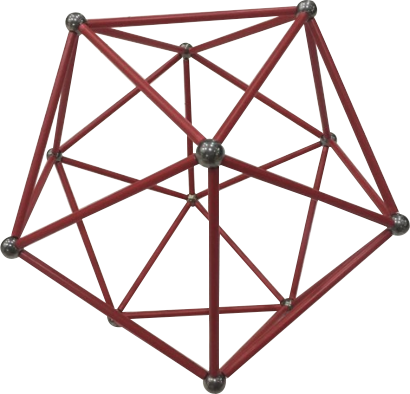
\includegraphics[width=0.25\textwidth]{1}
			\caption{\small\textit{Hình $1$}}
			\vspace*{-10pt}
		\end{figure}
		\begin{figure}[H]
			\centering
%			\vspace*{5pt}
			\captionsetup{labelformat= empty, justification=centering}
			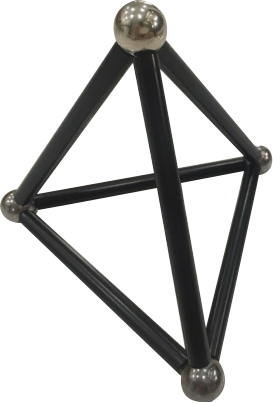
\includegraphics[width=0.23\textwidth]{2}
			\caption{\small\textit{Hình $2$}}
			\vspace*{-5pt}
		\end{figure}
	\end{multicols}
	
	\textbf{Câu hỏi $\pmb{1}$:} \textit{a. Nhìn vào hình vẽ và cho biết Bi đã dùng bao nhiêu viên bi và bao nhiêu thanh màu đen để ghép được Hình $2$?
	\vskip 0.1cm
	b. Có tất cả bao nhiêu tam giác có các cạnh là các thanh màu đen? }
	\begin{multicols}{2}
		Quá là đơn giản nhỉ? Hình kim tự tháp có đáy là hình tam giác này có $4$ đỉnh và $6$ cạnh, nên để ghép hình đó, Bi đã dùng $4$ viên bi và $6$ thanh màu đen.
		\begin{figure}[H]
			\centering
			\vspace*{5pt}
			\captionsetup{labelformat= empty, justification=centering}
			
\includegraphics[width=0.35\textwidth]{3}
			\caption{\small\textit{Hình $3$ -- Kim tự tháp tam giác}}
			\vspace*{-5pt}
		\end{figure}
	\end{multicols}	
	Bây giờ, để đếm số tam giác, đó chính là số mặt của kim tự tháp, nên chúng mình dễ dàng biết được là trong hình có $4$ tam giác có cạnh là các thanh màu đen, ứng với $4$ mặt của hình kim tự tháp.
	\vskip 0.1cm
	Hình tiếp theo mà Bi đố các bé không còn đơn giản như thế nữa đâu, chúng mình cần phải quan sát kỹ hơn đó.
	\vspace*{-5pt}
	\begin{multicols}{2}
		\begin{figure}[H]
			\centering
			\vspace*{5pt}
			\captionsetup{labelformat= empty, justification=centering} 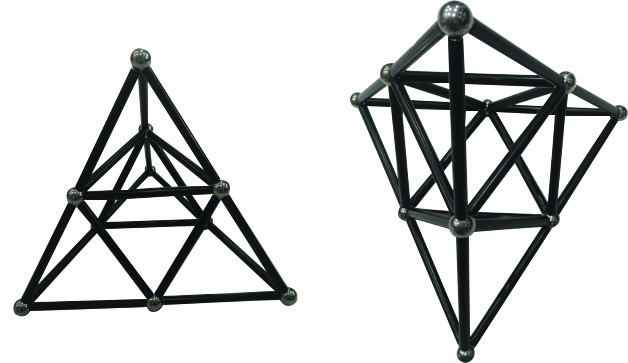
\includegraphics[width=0.35\textwidth]{4}
			\caption{\small\textit{Hình $4$}}
			\vspace*{-5pt}
		\end{figure}
		Trong Hình $4$ có hai góc nhìn khác nhau của cùng một khối hình. Nhìn có vẻ khó quan sát hơn rồi ấy nhỉ? Chúng mình cùng quan sát và tìm cách trả lời câu hỏi sau nhé.
	\end{multicols}
	\vspace*{-5pt}
	\textbf{Câu hỏi $\pmb{2}$:} \textit{Để xếp Hình $4$, Bi đã dùng tất cả bao nhiêu viên bi và bao nhiêu thanh đen?}
	\vspace*{-5pt}
	\begin{multicols}{2}
		Để trả lời câu hỏi này, Bi cũng rất suy nghĩ đấy. Dĩ nhiên là nếu phá bỏ khối hình và ngồi đếm từ từ thì quá đơn giản rồi. Nhưng đó đâu còn thú vị và thử thách nữa. Sau một hồi quan sát, thì Bi đã ló ra một ý tưởng để đếm số viên bi, đó là hãy đếm theo từng tầng. Bi đã chia khối hình thành ba tầng như Hình $5$.
		\begin{figure}[H]
			\centering
			\vspace*{-5pt}
			\captionsetup{labelformat= empty, justification=centering} 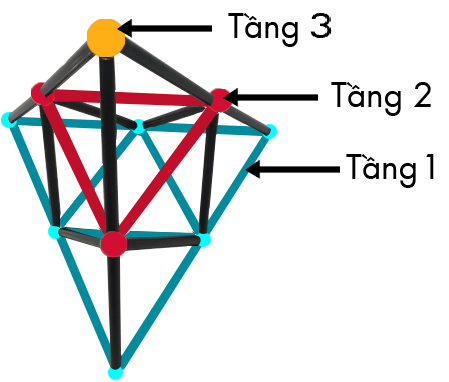
\includegraphics[width=0.32\textwidth]{5}
			
			\vspace*{-10pt}
			\caption{\small\textit{Hình $5$}}
			\vspace*{-5pt}
		\end{figure}
	\end{multicols}
	Bây giờ thì các bé đã thấy câu trả lời chưa? Từ  Hình $6$, chúng mình dễ dàng đếm được tầng $3$ thì chỉ có $1$ viên bi, tầng $2$ thì có $1+2 = 3$ viên bi, còn tầng $1$ thì có nhiều nhất là $1 + 2 + 3 = 6$ viên bi. Thế nên tổng cộng Bi đã dùng:
	$1 + 3 + 6 = 10 \text{ (viên bi)}.$
	\begin{multicols}{2}
		\begin{figure}[H]
			\centering
			\vspace*{15pt}
			\captionsetup{labelformat= empty, justification=centering} 
\includegraphics[width=0.475\textwidth]{6}
			\caption{\small\textit{Hình $6$}}
			\vspace*{-5pt}
		\end{figure}
		Nhưng còn để đếm số thanh đen thì không chỉ đơn giản như vậy nữa, đã phức tạp hơn rất nhiều rồi đấy. Có rất nhiều cách để đếm khác nhau, nhưng để Bi giới thiệu với các bé hai cách Bi đã tìm ra nhé.
	\end{multicols}
	\vskip 0.1cm
	\textbf{Cách $1$:} Khối hình này cũng là một kim tự tháp, nhưng mà là kim tự tháp to hơn Hình $2$. Khối hình này cũng có $6$ cạnh, mỗi cạnh cần $2$  thanh để ghép thành, ví dụ như phần được tô màu xanh trong Hình $7$. Vậy để làm thành các cạnh của khối kim tự tháp, Bi đã dùng:
	$ 2\times 6 = 12 \text{ (thanh đen)}.$
	\begin{multicols}{2}
		\begin{figure}[H]
			\centering
			\vspace*{5pt}
			\captionsetup{labelformat= empty, justification=centering} 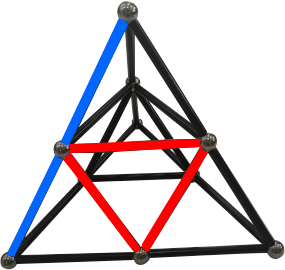
\includegraphics[width=0.3\textwidth]{7}
			\caption{\small\textit{Hình $7$}}
			\vspace*{-10pt}
		\end{figure}
		Nhưng như thế chưa đủ số thanh. Khối hình này có $4$ mặt, và mỗi mặt thì đều như tầng $1$ của Hình $6$. Ngoài các thanh đã dùng để xếp cạnh của kim tự tháp, mỗi mặt còn cần thêm $3$ thanh được tô màu đỏ để xếp nữa. Vậy tức là Bi cần dùng thêm $3 \times 4 = 12$ thanh màu đen để xếp các phần ở các mặt của kim tự tháp trong Hình $4$ mà không phải là cạnh.
	\end{multicols}
	\vskip 0.1cm
	Các bé thử quan sát xem vậy là đã đủ hết chưa nhỉ? Bi sẽ bật mí cho các bé rằng đã đủ hết số  thanh cần dùng rồi đó. Để xếp được hình ba tầng, Bi đã dùng tổng cộng:
	$ 12 + 12 = 24 \text{ (thanh đen)}.$
	\vskip 0.1cm
	\textbf{Cách $2$:} Những tưởng tìm được cách đếm này là đã đủ để hài lòng, thế nhưng Bi đã tìm ra cách đếm khác nữa đấy, vì cách đếm thứ hai này giúp Bi dễ dàng đếm với những hình nhiều tầng hơn nữa cơ.
	\vskip 0.1cm
	Chúng mình cùng quan sát lại khối hình và sẽ nhìn thấy hình $3$ tầng thật ra có rất nhiều hình kim tự tháp nhỏ bên trong đấy. Nhìn vào hình $8$, mình chia ra hình kim tự tháp đầu tiên có một mặt đáy là tầng $2$ (các cạnh màu đỏ), và có $3$ kim tự tháp có các mặt đáy là các tam giác thuộc tầng $3$. Và khối hình đã được chia ra làm $4$ kim tự tháp, các cạnh màu đen đều được xuất hiện đầy đủ trong cách chia này. Vậy nên ta có cách để tính số thanh đã dùng để xếp là: 
	$$4 \times 6 = 24 \text{ (thanh đen)}.$$	
	\begin{multicols}{2}
		Hình bên trái tô màu hình kim tự tháp trên cùng $- 4$ cạnh màu đỏ. Hình bên phải tô màu $3$ cái kim tự tháp bên dưới, mỗi cái một màu.
		\vskip 0.1cm
		Bi đã thử lại bằng cách dỡ bỏ khối hình ra và đếm lại rồi đấy, thật là chính xác luôn. Các bé cũng có thể thử bằng cách dùng các thanh gỗ và tre để thay thế cho các thanh đen, và dùng kẹo dẻo hoặc đất nặn thay cho các viên bi.
		\begin{center}
			\centering
			\vspace*{-10pt}
			\captionsetup{labelformat= empty, justification=centering} 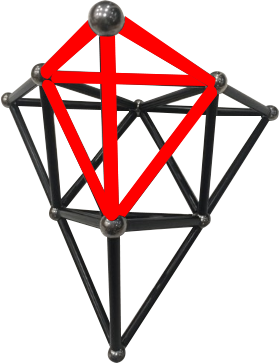
\includegraphics[width=0.2\textwidth]{8}\quad
			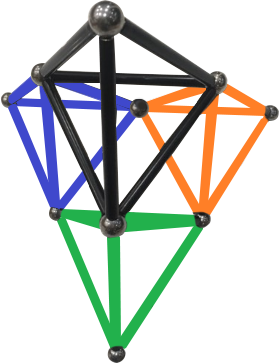
\includegraphics[width=0.2\textwidth]{8a}
			\textit{\small Hình $8$}
%			\vspace*{-5pt}
		\end{center}
	\begin{figure}[H]
		\centering
		\vspace*{-15pt}
		\captionsetup{labelformat= empty, justification=centering} 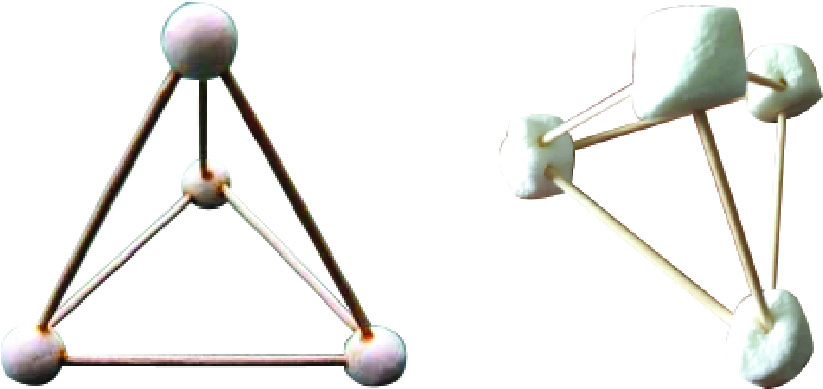
\includegraphics[width=0.42\textwidth]{9}
		\caption{\small\textit{Hình $9$}}
		\vspace*{-5pt}
	\end{figure}
	\end{multicols}
	\vspace*{-5pt}
	Bây giờ, các bé hãy cùng thử sức với một câu hỏi khó hơn nhé.
	\vskip 0.1cm
	\textbf{Câu hỏi $\pmb{3}$:} \textit{Trong Hình $4$, có tất cả bao nhiêu tam giác có các cạnh là các thanh đen, trong đó mỗi cạnh là một thanh đen?}
%	\vspace*{-5pt}
	\vskip 0.1cm
%	\begin{multicols}{2}
	\begin{wrapfigure}{r}{0.25\textwidth}
		\centering
		\vspace*{-10pt}
		\captionsetup{labelformat= empty, justification=centering} 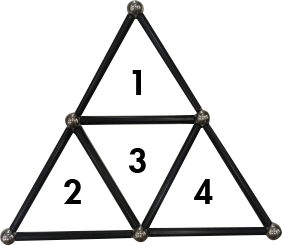
\includegraphics[width=0.22\textwidth]{10}
		\caption{\small\textit{Hình $10$}}
		\vspace*{-15pt}
	\end{wrapfigure}
	Ngày càng phức tạp nhỉ? Để tính số tam giác, đầu tiên thì Bi quan sát $4$ mặt của khối hình. Mỗi mặt sẽ có $4$ hình tam giác nhỏ:
	\vskip 0.1cm
	Vậy là ở mặt ngoài của hình kim tự tháp, chúng mình có tổng cộng:
	\vskip 0.1cm
	\hspace*{35pt}{$4 \times 4 = 16 \text{ (tam giác cạnh $1$)}.$}
	\vskip 0.1cm
	\vspace*{5pt}
	Nhưng như vậy đã đủ chưa nhỉ? Mình dễ lầm tưởng là hết rồi, nhưng sau khi quan sát rất kỹ thì Bi nhìn thấy còn các hình khác nữa cơ.
	\vskip 0.1cm
	\begin{wrapfigure}{l}{0.25\textwidth}
		\centering
		\vspace*{-15pt}
		\captionsetup{labelformat= empty, justification=centering} 
\includegraphics[width=0.23\textwidth]{11}
		\vspace*{-5pt}
		\caption{\small\textit{Hình $11$}}
		\vspace*{-20pt}
	\end{wrapfigure}
	\vspace*{-1pt}
	Các bé hãy nhìn lại Hình $5$, chúng mình sẽ thấy tầng $2$ chính là một tam giác cạnh $1$. Vấn đề là có bao nhiêu tam giác như vậy nhỉ? Có $4$ mặt của kim tự tháp và tương ứng sẽ có $4$ tam giác kiểu tam giác ở tầng $2$. Thế là chúng mình có thêm $4$ tam giác nữa.
	\vskip 0.15cm
	Vậy là cuối cùng, Bi đã đếm được có tất cả $20$ tam giác cạnh $1$ đấy.
	\vskip 0.1cm
	\textbf{Câu hỏi $\pmb{4}$:} \textit{Trong Hình $4$, có tất cả bao nhiêu tam giác có các cạnh là các thanh đen, tính cả các tam giác “to”, tức là có cạnh nhiều hơn một thanh đen?}
	\vspace*{-5pt}
	\begin{multicols}{2}
		Để tìm được đáp án của câu này sau khi đã biết câu $3$, thì vấn đề đơn giản hơn nhiều. Trong Hình $4$, chỉ có các tam giác có cạnh bằng $1$  thanh đen hoặc tam giác có cạnh bằng $2$ thanh đen mà thôi. Số tam giác có cạnh bằng $2$ thanh đen dễ đếm hơn rất nhiều, mỗi mặt có đúng một tam giác như vậy, nên có tất cả $4$ tam giác có cạnh bằng $2$ thanh đen.
		\begin{figure}[H]
			\centering
			\vspace*{-5pt}
			\captionsetup{labelformat= empty, justification=centering} 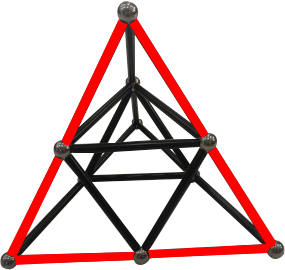
\includegraphics[width=0.3\textwidth]{12}
			\caption{\small\textit{Hình $12$}}
			\vspace*{-5pt}
		\end{figure}
	\end{multicols}
	Vậy là cuối cùng chúng mình đã tính được tổng số tam giác rồi đó, có $24$ tam giác các cỡ.
	\vskip 0.1cm
	Bây giờ, các bé hãy cùng thử sức với các câu hỏi tiếp theo nhé, khó hơn một chút đấy.
	\begin{multicols}{2}
	\textbf{Câu hỏi $\pmb{5}$:} \textit{a. Để xếp Hình $13$, Bi đã dùng tất cả bao nhiêu viên bi và bao nhiêu thanh đen? 
	\vskip 0.1cm
	b. Trong Hình $13$, có tất cả bao nhiêu tam giác có các cạnh là các thanh đen, tính cả các tam giác “to”, tức là có cạnh nhiều hơn một thanh đen?}
	\begin{figure}[H]
		\centering
		\vspace*{5pt}
		\captionsetup{labelformat= empty, justification=centering} 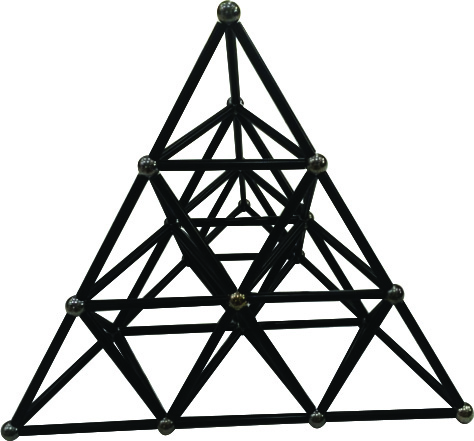
\includegraphics[width=0.2\textwidth]{13}
		\quad
		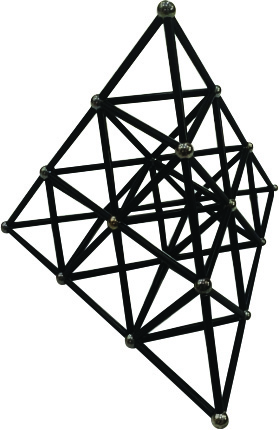
\includegraphics[width=0.2\textwidth]{13a}
		\caption{\small\textit{Hình $13$}}
		\vspace*{-5pt}
	\end{figure}
	\end{multicols}







